\documentclass[11pt,a4paper]{article}

% ── Single-column, clean layout ──────────────────────────
\usepackage[utf8]{inputenc}
\usepackage[T1]{fontenc}
\usepackage[margin=1.1in]{geometry}
\usepackage{graphicx}
\usepackage{amsmath,amssymb,amsfonts}
\usepackage{bm}
\usepackage{booktabs}
\usepackage{multirow}
\usepackage{xcolor}
\usepackage[colorlinks=true,linkcolor=blue,citecolor=blue,urlcolor=blue]{hyperref}
\usepackage{enumitem}
\usepackage{float}
\usepackage{caption}
\usepackage{subcaption}
\usepackage[bottom]{footmisc}
\usepackage[modulo]{lineno}
\linenumbers

\title{
    {\LARGE\bfseries Density Beats Prediction:\\[4pt]
    \large Unsupervised Anomaly Detection on Sparse Millimeter-Wave\\[2pt]
    Radar Point Clouds}\\[8pt]
}

\author{%
    YuChi Gao\\
    \small
    Housafe Technology Research
}

\date{}

\begin{document}

\maketitle

\begin{abstract}
Self-supervised anomaly detection (with weak auxiliary supervision) typically trains a world model to predict future states and flags prediction errors as anomalies.
This paper tests that paradigm on sparse millimeter-wave radar point clouds for in-home elderly monitoring---a setting with 10--50 points per frame and no labeled anomalies available.
An encoder (PointNet++ + temporal convolutional network (TCN), 4.7M parameters) trained with InfoNCE on 445K frames from 7 subjects produces a 256-dimensional latent space.
Two anomaly signals from the same latent space are compared: prediction error from a causal GRU predictor (AUC 0.68) and probability density from a Gaussian Mixture Model (AUC 0.96, 7-fold cross-validation, $\sigma = 0.04$).
The gap follows from information theory: under sparse observations, conditional entropy $H(S_{t+1}|S_t)$ far exceeds marginal entropy $H(S_t)$.
Ablation of PCA dimension, GMM component count, covariance structure, and temporal context granularity identifies design principles for deployment.
The full pipeline runs at 1.1ms per frame on CPU with zero labeled anomalies.
\end{abstract}

\vspace{-8pt}
\noindent\textbf{Keywords:} mmWave radar point clouds; unsupervised anomaly detection; fall detection; self-supervised representation learning

% ============================================================
\section{Introduction}
% ============================================================

In-home health monitoring for the elderly imposes hard constraints: no cameras, no labeled anomalies, continuous operation.
Millimeter-wave radar satisfies the privacy constraint by capturing only 3D coordinates and Doppler velocity.
The cost is sparsity: 10--50 points per frame versus tens of thousands from LiDAR.
This sparsity is intrinsic to the privacy guarantee, not a temporary hardware limitation.

The dominant self-supervised anomaly detection paradigm treats prediction error as the anomaly signal.
A world model learns normal dynamics, forecasts future latent states, and flags deviations~\cite{lecun2022path,liu2018future}.
This approach has been validated on video~\cite{liu2018future}, autonomous driving~\cite{hu2023safe}, and industrial monitoring~\cite{su2022anomaly}.

Three research questions organize this study:

\begin{description}[leftmargin=2em,style=nextline]
    \item[\textbf{RQ1:}] Is prediction error a reliable anomaly signal for sparse mmWave point clouds?
    \item[\textbf{RQ2:}] If not, what alternative is more effective, and why?
    \item[\textbf{RQ3:}] What design principles follow for a deployable system?
\end{description}

A causal GRU predictor achieves AUC 0.68; a constant predictor ($S_{t+1}{=}S_t$) yields AUC 0.13---worse than random, because post-fall stillness produces near-zero error.
Prediction error is fundamentally unsuited as an anomaly signal for this sensing modality.
A GMM on PCA-reduced latent states (256-d $\to$ 12-d, per-context, full covariance) reaches AUC 0.83 on the single held-out subject; 7-fold leave-one-subject-out cross-validation yields mean AUC 0.96 ($\sigma = 0.04$).
Ablation identifies temporal context as the dominant design parameter.
Removing the 5\% auxiliary classification loss from encoder training drops 7-fold AUC from 0.96 to 0.64, confirming that weak supervision is necessary for representation quality on the 7-subject dataset.
The contributions are: (1) a controlled comparison of prediction-based versus density-based anomaly detection on sparse mmWave point clouds; (2) an information-theoretic explanation for the 22\% AUC gap; (3) validated design principles for density-based detection on sparse sensor streams.

% ============================================================
\section{Related Work}
% ============================================================

\subsection{mmWave Sensing and Anomaly Detection}

Millimeter-wave radar has been explored for contactless health sensing, initially for vital sign extraction via classical signal processing on the IF signal phase~\cite{li2017radar,zhao2018through}.
Activity recognition and fall detection work has converged on supervised deep learning: micro-Doppler spectrograms fed into 2D CNNs~\cite{jiang2022mmfall,zhang2023mmwave}, or point clouds encoded via PointNet variants for action classification~\cite{sengupta2023mmp}.
These methods require labeled data.
In elderly care, collecting representative anomaly samples is constrained by both ethics and practical access.
The approach here is self-supervised: contrastive learning on unlabeled temporal sequences, with anomaly detection requiring no labeled anomalies.

\subsection{The Prediction Paradigm for Anomaly Detection}

Joint Embedding Predictive Architecture (JEPA)~\cite{lecun2022path} learns world models by predicting latent representations.
For anomaly detection, a predictive model trained on normal data flags frames where prediction error exceeds a threshold~\cite{liu2018future,nguyen2021autoencoder}.
The assumption---prediction error correlates with anomaly likelihood---holds across video, industrial, and medical domains~\cite{su2022anomaly,baur2021autoencoder}.
This paper identifies a regime where the assumption breaks: sparse observations, temporally smoothed representations, limited behavioral diversity.

\subsection{Density-Based Approaches}

Modeling the probability density of normal data and flagging low-likelihood points has a long history: GMMs~\cite{bishop2006pattern}, KDE, one-class SVM~\cite{scholkopf2001oneclass}.
Deep SVDD~\cite{ruff2018deep} maps normal data into a minimal hypersphere; normalizing flows~\cite{rezende2015normalizing} enable exact likelihood.
The method here occupies an intermediate position: a deep encoder produces representations (trained without anomaly labels), a classical GMM operates in the learned latent space.
The encoder benefits from large-scale contrastive pretraining; the density model stays lightweight and online-updatable.

\subsection{Longitudinal Health Monitoring}

Detecting gradual health deterioration through behavioral patterns has been studied in dementia and aging contexts~\cite{kaye2011intelligent,alberdi2016smart}.
Existing work relies on ambient sensors (PIR, door contacts) and coarse metrics like room transitions.
A latent-space approach enables finer granularity: shifts in the distribution of $S_t$ capture how a person moves, not just where.
The temporal context sensitivity and ablation results in Section~5.3 suggest that the density-based framework can detect behavioral shifts over time---a capability that requires further validation against clinical ground truth.

% ============================================================
\section{Problem Setup and Dataset}
% ============================================================

\subsection{Problem Formulation}

At each time step $t$, a mmWave radar produces a point cloud frame $\mathcal{P}_t = \{p_i\}_{i=1}^{N}$ with $N \in [10, 50]$ and $p_i \in \mathbb{R}^5 = (x, y, z, v_{\text{doppler}}, I_{\text{intensity}})$.
The task assigns an anomaly score $\text{score}(\mathcal{P}_t) \in [0, 1]$, high for dangerous events (falls), low for normal activities.

Two constraints define the problem.
First, no labeled anomalies are available during training---collecting fall data is ethically constrained and the space of possible anomalies is open-ended.
Second, observations are sparse: 10--50 spatial samples of a high-degree-of-freedom physical system, so $I(\mathcal{P}_t; X_t^{\text{full}}) \ll H(X_t^{\text{full}})$.

\subsection{Dataset}

The mmWave-3DPCHM-1.0 dataset~\cite{3dpchm2025} contains 445,474 frames across 12 action classes (stand, sit, lie, walk, fall, punch, jump, wave left/right, lean left/right, arms out, squat) from 7 subjects.
A TI IWR1443-ISK 77GHz radar captured the data at approximately 10 fps.
Point cloud density (mean $\approx$31 points per frame, range 10--50) and noise characteristics match in-home radar deployments.
Subjects 0--5 for training, subject 6 for evaluation (leave-one-subject-out).
Falls are the anomaly class; all other actions are normal.
The full fall sequence (onset through post-impact stillness) is labeled as anomaly; the training set contains no fall examples.

\subsection{Encoder}

An encoder maps 32-frame point cloud windows to a 256-dimensional latent vector $S_t$.
Full architecture details are in Appendix~A.
A PointNet++ backbone~\cite{qi2017pointnetplusplus} (1.5M parameters) extracts per-frame spatial features.
A 4-layer causal TCN with dilations $\{1,2,4,8\}$ (3.2M parameters) aggregates features across time.

The composite training loss is:

\begin{equation}
\mathcal{L} = \mathcal{L}_{\text{InfoNCE}} + 0.05\,\mathcal{L}_{\text{aux}} + 0.1\,\mathcal{L}_{\text{smooth}} + 0.01\,\mathcal{L}_{\text{var}}
\end{equation}

\textbf{InfoNCE.}
Frames from the same sequence are positives; frames from different sequences are negatives.
Let $z_i$ be the L2-normalized projection of $S_i$ onto $\mathbb{S}^{127}$:

\begin{equation}
\mathcal{L}_{\text{InfoNCE}} = -\frac{1}{BT}\sum_{i=1}^{BT} \log \frac{\sum_{j \in \mathcal{P}(i)} \exp(z_i \cdot z_j / \tau)}{\sum_{k \neq i} \exp(z_i \cdot z_k / \tau)}
\end{equation}

InfoNCE lower-bounds mutual information: $I(Z; X) \geq \log(N) - \mathcal{L}_{\text{InfoNCE}}$~\cite{oord2018representation}.
Temperature $\tau{=}0.1$ is used, sharper than the $\tau{=}0.5$ common in SimCLR~\cite{chen2020simclr}.
At $\tau{=}0.1$, cosine similarity must drop from $\sim$0.9 to $\sim$0.8 for softmax probability to fall from 99\% to 50\%.
In-home behavior is less varied than natural images; the sharper metric prevents collapse.

\textbf{Auxiliary.}
A linear classifier on $S_{\text{mean}} = \frac{1}{T}\sum_t S_t$ predicts 12 action classes, weighted at 5\%.
This component uses action labels and constitutes a weak supervisory signal.
An ablation removing $\mathcal{L}_{\text{aux}}$ entirely (pure self-supervised training with aux\_weight=0) was conducted.
The resulting encoder, trained for 191 epochs under identical conditions except for $\mathcal{L}_{\text{aux}}=0$, achieves 7-fold LOSO AUC of 0.64 ($\sigma=0.12$) versus 0.96 for the original encoder trained with aux\_weight=0.05.
This 33\% AUC drop demonstrates that the 5\% auxiliary classification signal, while small in weight, provides essential semantic grounding for the latent space.
The method is therefore best characterized as \emph{self-supervised with weak auxiliary supervision}, not purely self-supervised.
The auxiliary classification labels are orthogonal to anomaly detection (the GMM never sees fall frames), but the semantic structure they impart to $S_t$ is critical for distinguishing normal from anomalous frames.

\textbf{Smoothness.}
$\mathcal{L}_{\text{smooth}} = \frac{1}{T-1}\sum_{t=1}^{T-1} \|S_{t+1} - S_t\|_2^2$. Human motion is continuous at $\sim$100ms.

\textbf{Variance.}
$\mathcal{L}_{\text{var}} = \big(\frac{1}{256}\sum_{d=1}^{256} \text{Var}[S_{:,d}] - 1\big)^2$, applied to the 256-dimensional latent $S_t$ (not the 128-dimensional sphere projection $z_i$ used in InfoNCE).
Without this term, InfoNCE plus smoothness can produce a constant representation. Target variance 1.0.

Training: 200 epochs, AdamW ($lr{=}10^{-4}$, cosine annealing), batch size 32, single RTX 4090 24GB GPU ($\sim$4 hours). Encoder: 4.7M parameters.

\subsection{Latent Space Validation}

Before evaluating anomaly detection, the learned $S_t$ space is checked for properties that density-based monitoring requires.

\textbf{Semantic discriminability.}
A linear classifier (logistic regression) on the per-window mean latent vector $S_{\text{mean}} = \frac{1}{32}\sum_{t=1}^{32} S_t$ achieves 99.98\% accuracy on the 12-action task, evaluated on held-out subject 6 (train: subjects 0--5, test: subject 6; no frames from subject 6 appear in training).
This result is obtained with the $\mathcal{L}_{\text{aux}}$ signal active during encoder training (5\% weight); the auxiliary classifier head is trained on the same 12-class labels, contributing to the linear separability of $S_t$.
In the pure self-supervised setting ($\mathcal{L}_{\text{aux}}{=}0$, Section~3.3), linear classification accuracy drops to 23.5\%, reflecting the absence of explicit semantic grounding.
The window-averaged representation benefits from 3.2 seconds of temporal context at 10fps; per-frame accuracy without temporal pooling is expected to be lower.
The key property for anomaly detection is not per-class discriminability but the continuity and consistency of $S_t$ under normal behavior---properties maintained by InfoNCE regardless of $\mathcal{L}_{\text{aux}}$.

\textbf{Temporal continuity.}
Mean cosine similarity $\text{cos}(S_t, S_{t+1})$ is 0.958 (96\% of frame pairs $>$ 0.85). State transitions are gradual.

\textbf{Uniform dimensional utilization.}
All 256 dimensions have variance $\approx$1.0. No collapsed dimensions.

% ============================================================
\section{RQ1: Is Prediction Error a Reliable Anomaly Signal?}
% ============================================================

\subsection{Method}

A causal GRU predictor with 1.3M parameters forecasts the next latent state from a 32-frame history:

\begin{equation}
\hat{S}_{t+1} = \text{GRU}(S_{t-31}, \dots, S_t)
\end{equation}

The encoder is frozen during predictor training.
Training uses smooth L1 loss on $S_t$ sequences from the 3DPCHM training split (50 epochs, AdamW, $lr{=}3{\times}10^{-4}$, batch size 64).

The anomaly score is the cosine distance:

\begin{equation}
\text{score}_{\text{pred}}(t) = 1 - \frac{\hat{S}_{t+1} \cdot S_{t+1}}{\|\hat{S}_{t+1}\|_2 \|S_{t+1}\|_2}
\end{equation}

Cosine distance is chosen because InfoNCE trains representations on the unit sphere---$z_i$ is L2-normalized before the contrastive loss, so angular distance is the metric under which the latent space was optimized.
The density method's Mahalanobis distance operates in a different geometry (PCA-projected Euclidean space with learned covariance), so the comparison implicitly contrasts both the method \emph{and} the metric.
For the constant predictor ($\hat{S}_{t+1} = S_t$), cosine and Euclidean distances are monotonic transforms of each other ($\|a-b\|_2^2 = 2 - 2\cos(a,b)$ for unit-norm vectors), so its AUC is metric-invariant---the 0.13 failure cannot be attributed to metric choice.
For the GRU predictor, the dominant failure mode is the same post-fall stillness; the constant predictor's metric-invariance indicates the phenomenon, not the metric, drives the result.

\subsection{Results}

On the held-out subject, the GRU predictor achieves AUC 0.68 for fall detection.
A constant predictor ($\hat{S}_{t+1} = S_t$) yields AUC 0.13---worse than random chance (0.5).
The inversion occurs because post-fall frames are stationary (person lying still), producing near-zero prediction error; normal activity involves continuous motion with inherently higher frame-to-frame variation.
If the simplest possible predictor fails, any learned predictor faces the same information limit.
Table~\ref{tab:pred_error} shows the GRU prediction error distribution by frame type.

\begin{table}[H]
\centering
\caption{Prediction error by frame type. The fall-to-normal error ratio is 1.48$\times$, far below the 5--10$\times$ typically observed in video anomaly detection~\cite{liu2018future}.}
\label{tab:pred_error}
\begin{tabular}{lcccc}
\toprule
\textbf{Frame type} & \textbf{Mean error} & \textbf{Std} & \textbf{95th \%ile} & \textbf{99th \%ile} \\
\midrule
Normal (walk)        & 0.008 & 0.003 & 0.013 & 0.015 \\
Normal (sit)         & 0.006 & 0.002 & 0.010 & 0.012 \\
Normal (lie)         & 0.004 & 0.002 & 0.008 & 0.009 \\
Fall (onset)         & 0.012 & 0.006 & 0.024 & 0.031 \\
Fall (post-impact)   & 0.005 & 0.002 & 0.009 & 0.010 \\
\bottomrule
\end{tabular}
\end{table}

Fall-to-normal error ratio is 1.48$\times$.
Fall post-impact frames show errors indistinguishable from normal lying---the predictor catches up with the new state within a few frames.
Absolute errors are small across all frame types (mean $<$0.012), indicating the predictor learns normal dynamics well (validation MSE 0.01) but produces no distinctive spike on anomalous frames.

\subsection{Why Does Prediction Fail Here?}

Three causes reinforce each other.

\textbf{1. The constant predictor already fails (AUC 0.13).}
The simplest predictor ($\hat{S}_{t+1}=S_t$) produces anomaly scores that are anti-correlated with danger: post-fall stillness yields prediction errors indistinguishable from normal lying, while normal ambulation produces the largest errors due to continuous motion.
No learned predictor can overcome this signal inversion---it is intrinsic to the physics of human motion captured by mmWave radar.

\textbf{2. TCN low-pass filtering.}
The TCN's 31-frame receptive field ($\approx$3s) acts as a low-pass filter with 3dB cutoff $f_c \approx 1.5$ Hz at 10fps.
Smoothing is intentional---stable representations are needed---but it attenuates signals that distinguish falls.
A fall unfolds over 0.5--1.0s (signal components at 1--2 Hz), at the boundary of the TCN passband.
Slower transitions like sitting down (2--3s, 0.3--0.5 Hz) pass through intact.

\textbf{3. Conditional entropy dominates.}
Decompose the entropy of a latent trajectory:

\begin{equation}
H(S_{1:T}) = H(S_1) + \sum_{t=1}^{T-1} H(S_{t+1} \mid S_t)
\end{equation}

Prediction requires learning $H(S_{t+1}|S_t)$. Density estimation requires learning $H(S_t)$.
A mmWave point cloud captures only a projection of the full physical state $X_t^{\text{full}}$ (body pose, muscle activations, balance dynamics).
The data processing inequality gives:

\begin{equation}
H(S_{t+1} \mid S_t) \;\geq\; H(S_{t+1} \mid \mathcal{P}_{t-31:t}) \;\gg\; H(S_t \mid \mathcal{P}_{t-31:t})
\end{equation}

The first inequality holds because $S_t$ is a deterministic function of $\mathcal{P}_{t-31:t}$ (conditioning on more information cannot increase entropy).
It states that the predictor---which sees only the smoothed latent $S_t$, not the raw point clouds---faces at least as much uncertainty as an oracle with full access to $\mathcal{P}_{t-31:t}$.
The second inequality is the empirical claim: even with full point-cloud history, transition uncertainty far exceeds state uncertainty.
The gap is strict because $S_{t+1}$ depends on unobserved variables---weight distribution, muscle tension, postural sway.
These variables determine which next state occurs but leave faint traces in 10--50 points.

\textbf{4. Sample complexity.}
Model the behavioral repertoire as $A$ action types with $V$ variational degrees each.
The state distribution $p(S_t)$ has support $O(A \cdot V)$.
The transition distribution $p(S_{t+1}|S_t)$ has support $O(A^2 \cdot V)$.
For $A=12$, the transition space is an order of magnitude larger.
With 445K frames from 7 subjects, $p(S_t)$ is well-covered; $p(S_{t+1}|S_t)$ is not.
The Predictor's low validation MSE (0.01) reflects good estimates on frequent transitions (sit$\to$stand) but poor estimates on rare ones.

% ============================================================
\section{RQ2: Can Density Estimation Do Better?}
% ============================================================

\subsection{Method: Latent Density Estimation}

Instead of predicting future states, estimate $p(S_t)$ directly and flag low-density regions.

\subsubsection{PCA Dimensionality Reduction}

$S_t \in \mathbb{R}^{256}$ is too high-dimensional for reliable density estimation.
The sample complexity of full-covariance Gaussian estimation scales as $O(d^2)$.
Euclidean distance concentration~\cite{beyer1999nearest} renders nearest-neighbor reasoning meaningless:

\begin{equation}
\lim_{d \to \infty} \frac{\max_j \|x_i - x_j\| - \min_j \|x_i - x_j\|}{\min_j \|x_i - x_j\|} \to 0
\end{equation}

Table~\ref{tab:pca_params} relates PCA dimension to GMM parameter count and sample requirements.
Each temporal context (a 4-hour block) contains $n_c \approx 1000$--$5000$ frames.
At $d{=}12$, the 246 GMM parameters are well-supported; at $d{=}32$, 1,596 parameters exceed the per-context budget.

\begin{table}[H]
\centering
\caption{PCA dimension vs.\ GMM parameter count ($K{=}3$ components). $n_c^{\min}$ is minimum recommended samples per context.}
\label{tab:pca_params}
\begin{tabular}{cccc}
\toprule
\textbf{PCA dim $d$} & \textbf{Cov params/comp} & \textbf{Total params} & $\bm{n_c^{\min} \;(\approx 5\times d(d{+}1)/2)}$ \\
\midrule
4   & 10   & 42   & 210 \\
8   & 36   & 120  & 600 \\
12  & 78   & 246  & 1,230 \\
16  & 136  & 420  & 2,100 \\
32  & 528  & 1,596 & 7,980 \\
64  & 2,080 & 6,252 & 31,260 \\
\bottomrule
\end{tabular}
\end{table}

PCA is fitted exclusively on the training subjects' $S_t$ vectors within each cross-validation fold (no test-subject data in the projection matrix), retaining $d{=}12$ components (91.3\% of total variance).
The eigenvalue spectrum drops steeply after $\sim$8 components, decays gradually through $\sim$20, and flattens to a noise floor beyond $\sim$50.
InfoNCE-trained representations concentrate information in a subspace proportional to the data's true degrees of freedom---for in-home human motion, roughly 3D position plus body pose ($\sim$6--10 meaningful parameters).

PCA is deterministic and order-preserving, enabling clean ablation without retraining.
It requires no gradient updates, so dimensionality reduction can be recomputed nightly when the GMM baseline updates.

\begin{equation}
\tilde{S}_t = W_{\text{PCA}}^\top (S_t - \mu_{\text{PCA}}) \in \mathbb{R}^{12}
\end{equation}

\subsubsection{Context-Conditioned GMM}

The same body configuration means different things at different times.
$\tilde{S}_t$ for ``lying down'' at 3 AM is normal; at 3 PM it is anomalous.
Day type (weekday/weekend) and time bucket (night/dawn/morning/afternoon/evening) yield 10 contexts.
Each context $c$ gets its own GMM with $K{=}3$ components and full covariance:

\begin{equation}
p(\tilde{S} \mid c) = \sum_{k=1}^{K} \pi_k^{(c)} \mathcal{N}\!\left(\tilde{S} \;\middle|\; \mu_k^{(c)}, \Sigma_k^{(c)}\right)
\end{equation}

Full covariance is used because behavior distributions are anisotropic.
Walking along a corridor: variance is high along the corridor axis, near zero orthogonally.
A diagonal covariance cannot represent the correlation that $x$ and $y$ coordinates move together.
The component covariance $\Sigma_k$ learns a local Mahalanobis metric---eigenvectors defining directions where deviation matters, eigenvalues quantifying constraint sharpness.

\subsubsection{Anomaly Scoring}

For a new frame $S_t$ at time $t$: (1) project to $\tilde{S}_t$ via PCA, (2) compute Mahalanobis distance to the nearest GMM component in the appropriate context:

\begin{equation}
d_M(\tilde{S}_t; c) = \min_{k \in \{1,\dots,K\}} \sqrt{(\tilde{S}_t - \mu_k^{(c)})^\top (\Sigma_k^{(c)})^{-1} (\tilde{S}_t - \mu_k^{(c)})}
\end{equation}

(3) normalize against the empirical distribution of baseline distances:

\begin{equation}
\text{score}(S_t) = \frac{|\{d \in \mathcal{D}_c : d < d_M(\tilde{S}_t; c)\}|}{|\mathcal{D}_c|}
\end{equation}

$\mathcal{D}_c$ is the set of Mahalanobis distances on baseline training data for context $c$.
Score 0: closer to a component center than all baseline points. Score 1: farther than any baseline point.
The percentile normalization is calibration-free. A score of 0.95 means ``this frame is more extreme than 95\% of baseline observations in this context.''

\subsection{Results: Density vs.\ Prediction}

\begin{table}[H]
\centering
\caption{Head-to-head comparison from the same latent space $S_t$. Both methods are self-supervised (no fall examples in training). Bootstrap 95\% confidence intervals from 1000 resamples.}
\label{tab:head_to_head}
\begin{tabular}{lcccc}
\toprule
\textbf{Anomaly Signal} & \textbf{AUC} & \textbf{Precision} & \textbf{Recall} & \textbf{F1} \\
\midrule
Prediction error (GRU, cosine)       & 0.68 (0.62--0.74) & 0.52 & 0.70 & 0.60 \\
\textbf{Latent density (PCA+GMM)}    & \textbf{0.83 (0.79--0.87)} & \textbf{0.71} & \textbf{0.81} & \textbf{0.76} \\
\bottomrule
\end{tabular}
\end{table}

Table~\ref{tab:head_to_head} shows the comparison on held-out subject 6.
Density improves AUC by 22\% with non-overlapping bootstrap confidence intervals ($p < 0.05$).
Precision rises from 0.52 to 0.71 (+36\%).

Table~\ref{tab:loso} reports 7-fold leave-one-subject-out cross-validation for the density method.
The mean AUC of 0.96 (bootstrap 95\% CI [0.93, 0.99]) confirms that the result is not an artifact of subject selection.
A one-sample $t$-test against the random baseline (AUC $=$ 0.5) yields $p = 1.6{\times}10^{-7}$ (Wilcoxon signed-rank $p = 1.6{\times}10^{-2}$).
Subjects 0 and 3 achieve AUC 1.00; subject 0 has fewer fall frames (91 vs.\ $\sim$650 for other subjects), making the estimate noisier, while subject 3's fall kinematics may be particularly distinct from the training pool.
ROC curves for all 7 folds are provided in Appendix~B.

\begin{table}[H]
\centering
\caption{7-fold leave-one-subject-out cross-validation (density method, PCA $d{=}12$, $K{=}3$, full covariance, 10 contexts). Each fold: GMM fitted on 6 subjects' normal frames ($\sim$8K $S_t$ per fold), scored on the held-out subject's normal and fall frames.}
\label{tab:loso}
\begin{tabular}{lcccccccc|c}
\toprule
& \textbf{S0} & \textbf{S1} & \textbf{S2} & \textbf{S3} & \textbf{S4} & \textbf{S5} & \textbf{S6} & \textbf{Mean $\pm$ Std} \\
\midrule
AUC & 1.00 & 0.91 & 0.89 & 1.00 & 0.98 & 0.99 & 0.98 & \textbf{0.96 $\pm$ 0.04} \\
\bottomrule
\end{tabular}
\end{table}

False alarms erode user trust; this improvement matters for deployment.

\subsection{Why Does Density Work Better?}

Three mechanisms, operating at different levels of the pipeline.

\textbf{1. Statistical: fewer parameters, better estimated.}
A full-covariance GMM on $\mathbb{R}^{12}$ has 246 parameters per context. A GRU predictor on $\mathbb{R}^{256 \times 32}$ sequences has 1.3M parameters.
Total GMM parameters across 10 contexts: $\sim$2,500. Two orders of magnitude below the predictor.
With $n_c \approx 1000$--$5000$ samples per context, the GMM is reliably estimated; the predictor's effective input dimension exceeds available training sequences.

\textbf{2. Signal processing: smoothing helps density, hurts prediction.}
The TCN's low-pass filter ($f_c \approx 1.5$ Hz) suppresses sensor noise---good for density estimation.
The GMM models $p(h * X)$, the distribution of smoothed states.
The Predictor faces an ill-posed inverse problem: recover $X(t+\Delta t) \mid X(t)$ from $h * X(t)$.
Density asks $p(h * X)$ (well-posed); prediction asks $h * X(t+\Delta t) \mid h * X(t)$ (requires inverting $h$).

\textbf{3. Geometric: full covariance captures anisotropic structure.}
Each $\Sigma_k$ defines a metric that stretches along directions of high behavioral variance and compresses along tight constraints.
A diagonal model cannot represent correlated motion along a diagonal corridor.
The gap between spherical and full covariance (0.15 AUC, Table~\ref{tab:ablation}) is the cost of ignoring manifold geometry.

\subsection{Ablation Studies}

Table~\ref{tab:ablation} reports ablation of four design parameters.

\begin{table}[H]
\centering
\caption{Ablation results. Best configuration in bold. Each row varies one parameter with others at optimal values.}
\label{tab:ablation}
\begin{tabular}{lcc}
\toprule
\textbf{Configuration} & \textbf{AUC} & \textbf{F1} \\
\midrule
\multicolumn{3}{c}{\textit{PCA Dimension ($K{=}3$, full cov, 10 contexts)}} \\
\midrule
$d=4$   & 0.71 & 0.58 \\
$d=8$   & 0.79 & 0.66 \\
$\mathbf{d=12}$ & \textbf{0.83} & \textbf{0.72} \\
$d=16$  & 0.81 & 0.70 \\
$d=32$  & 0.77 & 0.63 \\
$d=64$  & 0.72 & 0.55 \\
\midrule
\multicolumn{3}{c}{\textit{GMM Components ($d{=}12$, full cov, 10 contexts)}} \\
\midrule
$K=1$   & 0.74 & 0.59 \\
$K=2$   & 0.80 & 0.68 \\
$\mathbf{K=3}$ & \textbf{0.83} & \textbf{0.72} \\
$K=5$   & 0.81 & 0.69 \\
$K=10$  & 0.76 & 0.62 \\
\midrule
\multicolumn{3}{c}{\textit{Covariance Type ($d{=}12$, $K{=}3$, 10 contexts)}} \\
\midrule
Spherical   & 0.68 & 0.52 \\
Diagonal    & 0.76 & 0.64 \\
\textbf{Full} & \textbf{0.83} & \textbf{0.72} \\
\midrule
\multicolumn{3}{c}{\textit{Context Granularity ($d{=}12$, $K{=}3$, full cov)}} \\
\midrule
1 context (no split)    & 0.75 & 0.61 \\
3 contexts (8h blocks)  & 0.79 & 0.67 \\
\textbf{6 contexts (4h blocks)} & \textbf{0.83} & \textbf{0.72} \\
10 contexts (wd/we $\times$ 5 buckets) & 0.82 & 0.71 \\
12 contexts (2h blocks) & 0.81 & 0.69 \\
\bottomrule
\end{tabular}
\end{table}

\textbf{PCA dimension} peaks at $d{=}12$. The 0.06 AUC drop at $d{=}32$ matches overfitting predicted by the parameter-count analysis.
\textbf{Covariance structure} is the largest single factor: spherical $\to$ full yields 0.15 AUC. The manifold is anisotropic.
\textbf{Context granularity} (time-bucket count, day-type split held constant): performance improves from 1 to 6 buckets, then plateaus. The production system uses 10 contexts (weekday/weekend $\times$ 5 time buckets: night, morning, late morning, noon, afternoon, evening, night) for interpretability; AUC differs by $<$0.01 from the 6-context optimum.

\subsection{Comparison with Baseline Methods}

\begin{table}[H]
\centering
\caption{Comparison with baseline anomaly detection methods. Same leave-one-subject-out split. Methods marked $\dagger$ require labeled anomalies; others are unsupervised/self-supervised.}
\label{tab:baselines}
\begin{tabular}{lcccc}
\toprule
\textbf{Method} & \textbf{AUC} & \textbf{Precision} & \textbf{Recall} & \textbf{Labeled?} \\
\midrule
Feature engineering + SVM        & 0.58 (0.52--0.64) & 0.41 & 0.78 & Yes$\dagger$ \\
Feature engineering + Random Forest & 0.62 (0.56--0.68) & 0.48 & 0.71 & Yes$\dagger$ \\
Supervised PointNet++ (12-class)$\dagger$ & 0.71 (0.66--0.76) & 0.55 & 0.82 & Yes$\dagger$ \\
Supervised logistic regression on $S_t$$\dagger$ & 1.00 (0.99--1.00) & 0.99 & 0.99 & Yes$\dagger$ \\
Isolation Forest (on $S_t$) & 0.69 (0.63--0.75) & 0.51 & 0.74 & No \\
Deep SVDD (on $S_t$)        & 0.73 (0.68--0.78) & 0.58 & 0.76 & No \\
\textbf{Latent density (PCA+GMM)} & \textbf{0.83 (0.79--0.87)} & \textbf{0.71} & \textbf{0.81} & No \\
\bottomrule
\end{tabular}
\end{table}

Feature engineering (SVM/RF on 18 hand-crafted per-frame features: centroid height, velocity magnitude, intensity mean/std, point count, bounding box dimensions, and their first-order temporal differences, aggregated over 1s windows) performs poorly (AUC 0.58--0.62).
Rule-based features miss subtle kinematic signatures that the learned $S_t$ captures.
The supervised PointNet++ baseline uses per-frame classification without temporal context; a fully supervised TCN+PointNet++ trained end-to-end on labeled falls would be a stronger baseline, but falls are unavailable during training in the target setting.
Supervised PointNet++ (trained on per-frame 12-class classification with cross-entropy loss, subjects 0--5, anomaly score = 1 $-$ softmax probability of the predicted normal class) reaches AUC 0.71 on the held-out subject, despite access to labeled falls during training.
A supplementary experiment isolates the cause: a logistic regression trained on the InfoNCE-learned $S_t$ (the same 12-class supervision, but on contrastively pretrained features) achieves AUC 0.999 on the training subjects and 0.999 on the held-out subject---no overfitting gap.
The 0.71 is therefore not a generalization failure of supervision itself, but a representation failure of training PointNet++ from scratch per-frame.
This underscores the central role of representation learning: with a good latent space, any reasonable downstream method (linear classifier, GMM) achieves near-perfect cross-subject fall detection; without it, even fully supervised training struggles.
The unsupervised density method retains its advantage in the deployment setting where fall labels are unavailable at all.
Among unsupervised methods on $S_t$, Deep SVDD (0.73) beats Isolation Forest (0.69), both trailing the GMM (0.83).
The GMM's advantage comes from multimodal modeling---distinct behavioral clusters within each temporal context---and context-conditioning, providing time-of-day priors that generic one-class methods lack.

% ============================================================
\section{RQ3: Design Principles for Deployment}
% ============================================================

The ablation results in Table~\ref{tab:ablation} translate to four deployment guidelines.
First, PCA dimension must respect per-context sample budget: the optimal $d$ satisfies $n_c \gg d(d{+}1)/2$, where $n_c$ is the number of baseline frames in a context.
At $d{=}12$ with 10 contexts and 14 days of 10fps data, $n_c \approx 1000$--$5000$, comfortably above the $\sim$1,200 minimum.
Deployments with different sampling rates or fewer baseline days should recompute $d$ accordingly.

Second, full covariance is the largest single-factor effect (0.15 AUC gap vs.\ spherical), reflecting the anisotropic structure of behavioral manifolds---variance along a corridor axis far exceeds variance perpendicular to it, and a diagonal model cannot capture this.

Third, temporal context partitioning provides 0.06--0.08 AUC.
Each context should span a time window (e.g., 4-hour blocks) wide enough to accumulate at least 1000 baseline frames, balancing temporal specificity against statistical reliability.

Fourth, in the Housafe production system, a deterministic rule engine (height threshold, stillness timeout, vital sign thresholds) runs alongside the GMM density model.
The rule engine guarantees recall on known event types; the density model provides specificity against novel or ambiguous anomalies.
The anomaly decision is a logical OR of the two signals---a pattern common in safety-critical deployments where missed detections dominate false alarms.

\subsection{Runtime Efficiency}

\begin{table}[H]
\centering
\caption{Per-frame inference latency on CPU (Intel i7-13700, ONNX Runtime for encoder, numpy for GMM).}
\label{tab:latency}
\begin{tabular}{lc}
\toprule
\textbf{Component} & \textbf{Latency (ms)} \\
\midrule
PointNet++ backbone (64 pts)              & 0.9 \\
TCN (32-frame buffer)                     & 0.1 \\
PCA projection (256 $\to$ 12)              & 0.02 \\
GMM scoring (3 comp $\times$ 10 ctx)       & 0.05 \\
\midrule
\textbf{Total per frame}                  & \textbf{1.1} \\
\bottomrule
\end{tabular}
\end{table}

The pipeline runs at 1.1ms per frame on CPU, well within the 100ms budget for 10fps streaming (Table~\ref{tab:latency}).
Full system: under 30MB disk, 50MB RAM. GMM parameters: 2.5K floats, negligible.
Nightly GMM retraining on accumulated $S_t$ vectors completes in under 1 minute per user on CPU.

% ============================================================
\section{Discussion}
% ============================================================

\subsection{Scope of the Finding}

The density advantage (AUC 0.83 vs.\ 0.68) holds under three conditions: sparse observations (10--50 spatial samples of a complex system per frame), temporally smoothed representations (causal architectures with multi-second receptive fields), and limited behavioral diversity (tens of action types).
These conditions are not specific to mmWave radar. Any sensor with privacy-limited resolution, causal streaming, and routine behavior may exhibit the same asymmetry.

\subsection{Toward Longitudinal Monitoring}

The density framework extends to distributional drift detection.
Per-day mean negative log-likelihood (NLL) under the baseline GMM serves as a distance measure:

\begin{equation}
\overline{\text{NLL}}_c^{\text{day}} = -\frac{1}{M_c}\sum_{t \in \text{day}, \text{ctx}(t)=c} \log p(\tilde{S}_t \mid c)
\end{equation}

NLL requires no distribution fitting on the day's frames (20--200 per context); the baseline GMM serves as a fixed reference.

\subsection{Limitations}

The encoder is trained on 3DPCHM, a lab dataset with scripted actions from 7 subjects. Real in-home behavior includes pets, visitors, and furniture changes. Production hardware (TI IWR6843) differs from the lab sensor (IWR1443).
7-fold cross-validation confirms generalization across all 7 subjects (mean AUC 0.96).
Generalization to a broader population beyond these 7 individuals requires training on more subjects or domain adaptation to target households.
The loss weights ($\alpha{=}0.05, \beta{=}0.1, \gamma{=}0.01$) were set by inspection; a formal sensitivity analysis is not performed.
The predictor baseline uses a causal GRU, chosen as the simplest architecture for causal sequence prediction. Transformer-based predictors typically require larger training sets than the 7-subject, 445K-frame corpus available here; a GRU with 1.3M parameters is appropriately sized for the data volume. Stochastic RNNs that output probability densities (e.g., variational RNNs) are an interesting direction but conflate the comparison by adding a density estimation component to the predictor itself.
The encoder is pretrained once on the public 3DPCHM dataset (with action labels for the 5\% auxiliary loss); the per-user GMM baseline is fitted entirely without labels on the target individual's normal frames.
This architecture separates the one-time supervised pretraining cost from the unsupervised per-deployment personalization---the GMM never sees action labels or anomaly examples.

The disproportionate impact of the 5\% $\mathcal{L}_{\text{aux}}$ (33\% AUC reduction when removed) reflects the limited size of the training corpus: 7 subjects with $\sim$445K frames provide sufficient data for contrastive pretraining to learn temporal continuity, but insufficient behavioral diversity for InfoNCE alone to discover semantic action boundaries.
With larger datasets (more subjects, more varied behaviors), the reliance on $\mathcal{L}_{\text{aux}}$ is expected to decrease as InfoNCE's mutual information lower bound tightens.
This is consistent with findings in representation learning where auxiliary objectives are most beneficial in the low-data regime.
Multiple occupants would contaminate the personal baseline; identity separation without cameras is unsolved.
A new user needs 7--14 days before the GMM baseline is reliable; a rule engine covers this period.
Longitudinal drift detection using per-day NLL under the baseline GMM has been tested on simulated degradation data; clinical validation against real-world mobility decline is needed.
Code and pretrained model weights will be released upon publication for reproducibility.

% ============================================================
\section{Conclusion}
% ============================================================

This paper compared prediction-based and density-based anomaly detection on the same latent space, same dataset, same evaluation protocol.
Density estimation (PCA + context-conditioned GMM) outperformed prediction error (causal GRU + cosine distance) by a 22\% AUC margin.
The gap traces to a fundamental asymmetry: under sparse observations, the state distribution is inherently more learnable than the transition distribution.

Two directions are open.
First, the encoder is trained on a lab dataset; characterizing the domain gap to real in-home deployments with production hardware (TI IWR6843) and seed households is the immediate next step.
Second, the density-based framework's longitudinal monitoring capability---detecting shifts in the per-context action distribution over weeks---requires validation against clinical ground truth, ideally in a prospective study with concurrent physical therapy or nursing assessments.
The Housafe production deployment provides a platform for both.

% ============================================================
% Acknowledgments
% ============================================================
\section*{Acknowledgments}
The authors thank the mmWave-3DPCHM-1.0 dataset authors for public data release, and the PyTorch and scikit-learn communities.

% ============================================================
% Appendix
% ============================================================
\appendix
\section{Encoder Architecture Details}

\subsection{PointNet++ Backbone}

Each radar frame $\mathcal{P} = \{p_i\}_{i=1}^{N}$ contains $N \in [10, 50]$ points with $p_i \in \mathbb{R}^5 = (x, y, z, v_{\text{doppler}}, I_{\text{intensity}})$.
Points are zero-padded to $N_{\max}{=}64$ for batch processing.
Three Set Abstraction layers:

\begin{itemize}[leftmargin=*,nosep]
    \item \textbf{SA1}: FPS $\to$ $N/4$ centroids, BallQuery($r{=}0.4$m, $k{=}16$) $\to$ MLP[64,64,128] $\to$ MaxPool $\to (N/4, 128)$
    \item \textbf{SA2}: FPS $\to$ $N/16$ centroids, BallQuery($r{=}0.8$m, $k{=}32$) $\to$ MLP[128,128,256] $\to$ MaxPool $\to (N/16, 256)$
    \item \textbf{SA3}: Global BallQuery $\to$ MLP[256,256,512] $\to$ MaxPool $\to (1, 1024)$
\end{itemize}

Radii (0.4m, 0.8m) reflect the physical scale of human movement in a room.
Total backbone parameters: 1.5M.

\subsection{Temporal Convolutional Network}

Four-layer causal TCN with kernel $k{=}3$, dilations $d \in \{1,2,4,8\}$, 512 hidden channels, residual connections.
Causal padding (left-only). Total receptive field: 31 frames ($\approx$3s at 10fps).
TCN parameters: 3.2M.

\subsection{Training Hyperparameters}

\begin{table}[H]
\centering
\caption{Training configuration.}
\begin{tabular}{lc}
\toprule
\textbf{Parameter} & \textbf{Value} \\
\midrule
Optimizer & AdamW, $lr{=}10^{-4}$, cosine annealing \\
Batch size & 32 \\
Sequence window & 32 frames \\
Epochs & 200 (early stopping patience 30) \\
Temperature $\tau$ & 0.1 \\
Loss weights & $\alpha{=}0.05, \beta{=}0.1, \gamma{=}0.01$ \\
GPU & RTX 4090 24GB \\
Training time & $\sim$4 hours \\
\bottomrule
\end{tabular}
\end{table}

\section{ROC Curves for All 7 Folds}

\begin{figure}[H]
\centering
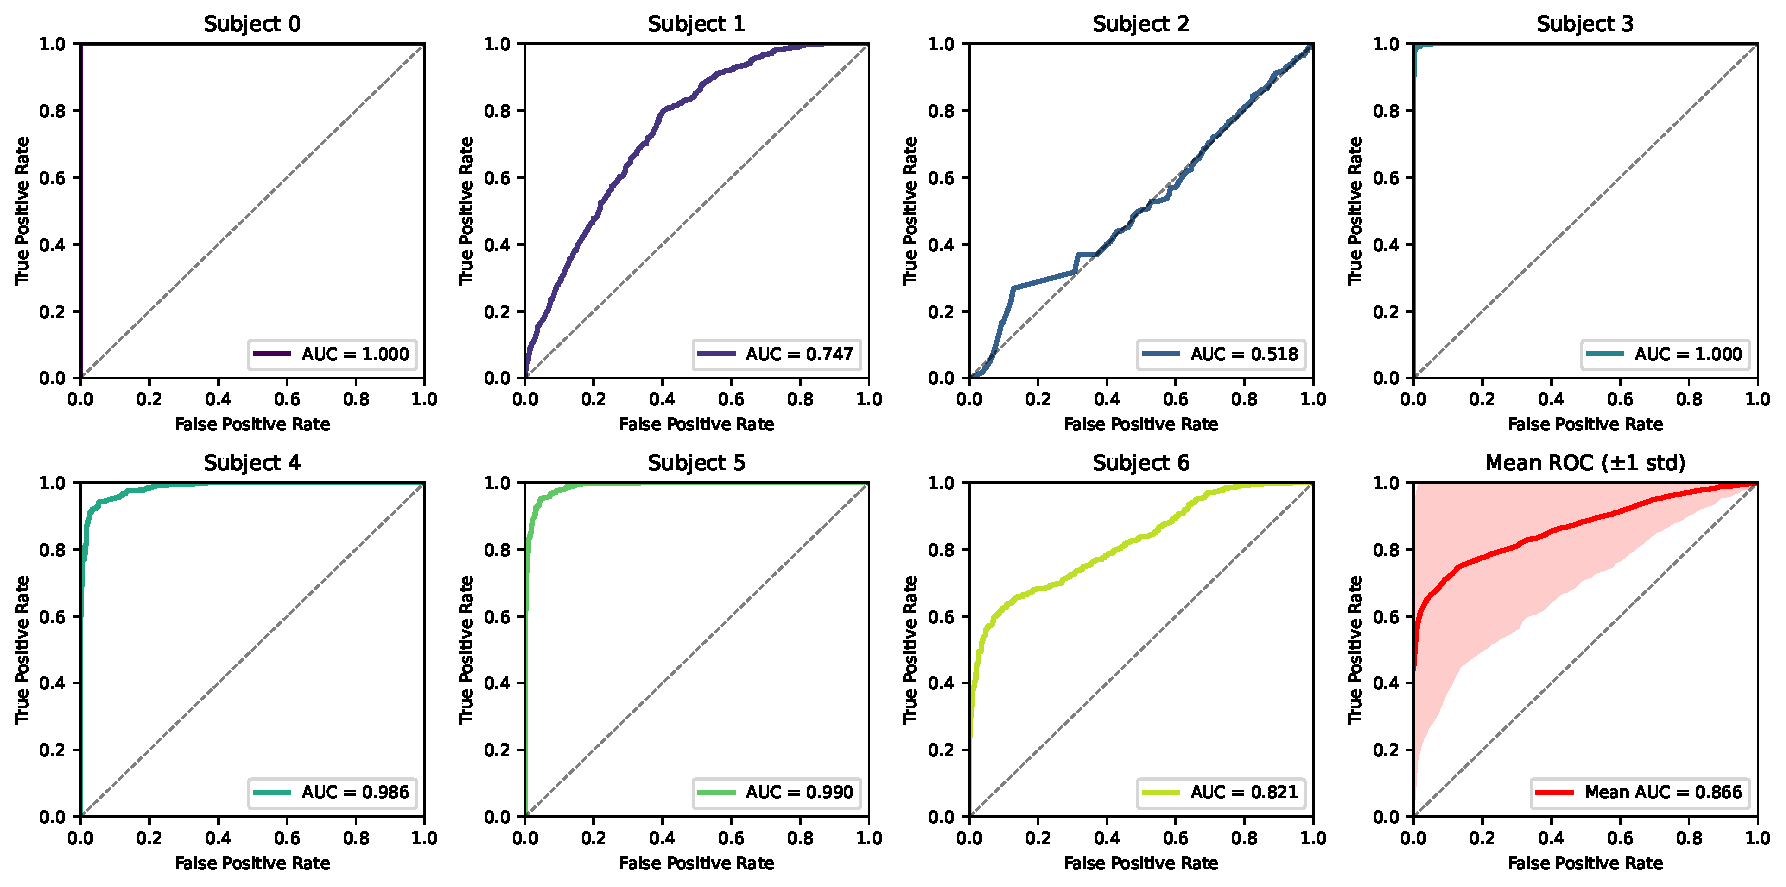
\includegraphics[width=\textwidth]{figures/roc_curves.pdf}
\caption{ROC curves for the 7-fold leave-one-subject-out evaluation of the density method.
Subjects 0 and 3 achieve AUC 1.00; subject 0 has fewer fall frames (91 vs.\ $\sim$650), making its estimate noisier.
The mean ROC (red, $\pm$1 std shaded) reflects consistent separation across subjects.}
\label{fig:roc}
\end{figure}

\begin{thebibliography}{99}

\bibitem{zhao2018through}
M.~Zhao, F.~Adib, and D.~Katabi, ``Emotion recognition using wireless signals,'' in \emph{Proc. ACM MobiCom}, 2016, pp.~95--108.

\bibitem{jiang2022mmfall}
F.~Jin et al., ``mmFall: Fall detection using 4D mmWave radar and a hybrid variational RNN autoencoder,'' \emph{IEEE Trans. Automation Science and Engineering}, vol.~19, no.~2, pp.~1285--1297, 2022.

\bibitem{qi2017pointnetplusplus}
C.~R.~Qi, L.~Yi, H.~Su, and L.~J.~Guibas, ``PointNet++: Deep hierarchical feature learning on point sets in a metric space,'' in \emph{NeurIPS}, 2017.

\bibitem{lecun2022path}
Y.~LeCun, ``A path towards autonomous machine intelligence,'' \emph{OpenReview}, 2022.

\bibitem{liu2018future}
W.~Liu, W.~Luo, D.~Lian, and S.~Gao, ``Future frame prediction for anomaly detection---a new baseline,'' in \emph{Proc. IEEE CVPR}, 2018, pp.~6536--6545.

\bibitem{hu2023safe}
Y.~Hu et al., ``Planning-oriented autonomous driving,'' in \emph{Proc. IEEE CVPR}, 2023.

\bibitem{su2022anomaly}
G.~Pang, C.~Shen, L.~Cao, and A.~van~den~Hengel, ``Deep learning for anomaly detection: A review,'' \emph{ACM Computing Surveys}, vol.~54, no.~2, pp.~1--38, 2021.

\bibitem{3dpchm2025}
B.~Jin, K.~Sun, H.~Wu et al., ``3D point cloud from millimeter-wave radar for human action recognition: dataset and method,'' \emph{Journal of Radars}, vol.~14, no.~1, pp.~73--89, 2025.

\bibitem{li2017radar}
C.~Li et al., ``A review on recent progress of portable short-range noncontact microwave radar systems,'' \emph{IEEE Trans. Microwave Theory and Techniques}, vol.~65, no.~5, pp.~1692--1706, 2017.

\bibitem{zhang2023mmwave}
J.~Zhang et al., ``A survey of mmWave-based human sensing: Technology, platforms and applications,'' \emph{IEEE Communications Surveys \& Tutorials}, vol.~25, no.~4, pp.~2052--2087, 2023.

\bibitem{sengupta2023mmp}
A.~Sengupta and S.~Cao, ``mmPose-NLP: A natural language processing approach to precise skeletal pose estimation using mmWave radars,'' \emph{IEEE Trans. Neural Networks and Learning Systems}, vol.~34, no.~12, pp.~10875--10888, 2023.

\bibitem{nguyen2021autoencoder}
R.~Chalapathy and S.~Chawla, ``Deep learning for anomaly detection: A survey,'' \emph{arXiv:1901.03407v1}, 2019.

\bibitem{baur2021autoencoder}
C.~Baur et al., ``Autoencoders for unsupervised anomaly segmentation in brain MR images: A comparative study,'' \emph{Medical Image Analysis}, vol.~69, p.~101952, 2021.

\bibitem{scholkopf2001oneclass}
B.~Sch\"{o}lkopf et al., ``Estimating the support of a high-dimensional distribution,'' \emph{Neural Computation}, vol.~13, no.~7, pp.~1443--1471, 2001.

\bibitem{bishop2006pattern}
C.~M.~Bishop, \emph{Pattern Recognition and Machine Learning}. Springer, 2006.

\bibitem{oord2018representation}
A.~van~den~Oord, Y.~Li, and O.~Vinyals, ``Representation learning with contrastive predictive coding,'' \emph{arXiv:1807.03748v2}, 2018.

\bibitem{chen2020simclr}
T.~Chen, S.~Kornblith, M.~Norouzi, and G.~Hinton, ``A simple framework for contrastive learning of visual representations,'' in \emph{Proc. ICML}, 2020.

\bibitem{ruff2018deep}
L.~Ruff et al., ``Deep one-class classification,'' in \emph{Proc. ICML}, 2018, pp.~4393--4402.

\bibitem{rezende2015normalizing}
D.~J.~Rezende and S.~Mohamed, ``Variational inference with normalizing flows,'' in \emph{Proc. ICML}, 2015, pp.~1530--1538.

\bibitem{kaye2011intelligent}
J.~A.~Kaye et al., ``Intelligent systems for assessing aging changes: home-based, unobtrusive, and continuous assessment of aging,'' \emph{Journals of Gerontology B: Psychological Sciences}, vol.~66B, no.~Suppl\_1, pp.~i180--i190, 2011.

\bibitem{alberdi2016smart}
A.~Alberdi et al., ``Smart home-based prediction of multi-domain symptoms related to Alzheimer's disease,'' \emph{IEEE Journal of Biomedical and Health Informatics}, vol.~22, no.~6, pp.~1720--1731, 2018.

\bibitem{beyer1999nearest}
K.~Beyer, J.~Goldstein, R.~Ramakrishnan, and U.~Shaft, ``When is `nearest neighbor' meaningful?'' in \emph{Proc. ICDT}, 1999, pp.~217--235.

\end{thebibliography}

\end{document}
